\documentclass{beamer}
\mode<presentation>

\usepackage{enumerate}

\title{Young Tableaux: una implementazione}
\author[Campagni]{Candidato: Alessandro Campagni \medskip \\Relatore:
  Marco Maggesi}
\date{}

\usetheme{CambridgeUS}

\begin{document}

\begin{frame}
\titlepage
\end{frame}

%% \frame{\tableofcontents}

\section{Preliminari}
\subsection{Diagrammi di Young}

\begin{frame}
\frametitle{Diagramma di Young}
\begin{columns}[T]
\column{5cm}
$11=4+3+2+1+1$\\
\vspace{1cm}
\includegraphics[width=0.6\textwidth]{images/YoungDiagram.pdf}
\column{5cm}
\begin{enumerate}[(i)]
\item lunghezza delle righe non crescente
\end{enumerate}
\end{columns}
\end{frame}

%% \begin{frame}
%% \frametitle{Diagramma coniugato}
%% \begin{columns}[T]
%% \column{5cm}
%% \includegraphics[height=0.6\textwidth]{images/YoungDiagramTransposed.pdf}
%% \column{5cm}
%% $11=5+3+2+1$
%% \end{columns}
%% \end{frame}

%% \begin{frame}
%% \frametitle{Skew diagram}
%% \centering
%% \begin{columns}
%% \begin{column}{3.3cm}
%% \includegraphics[width=0.7\textwidth]{images/skew_diag_1.pdf}\\
%% $\lambda=(5,3,2)$
%% \end{column}
%% \begin{column}{3.3cm}
%% 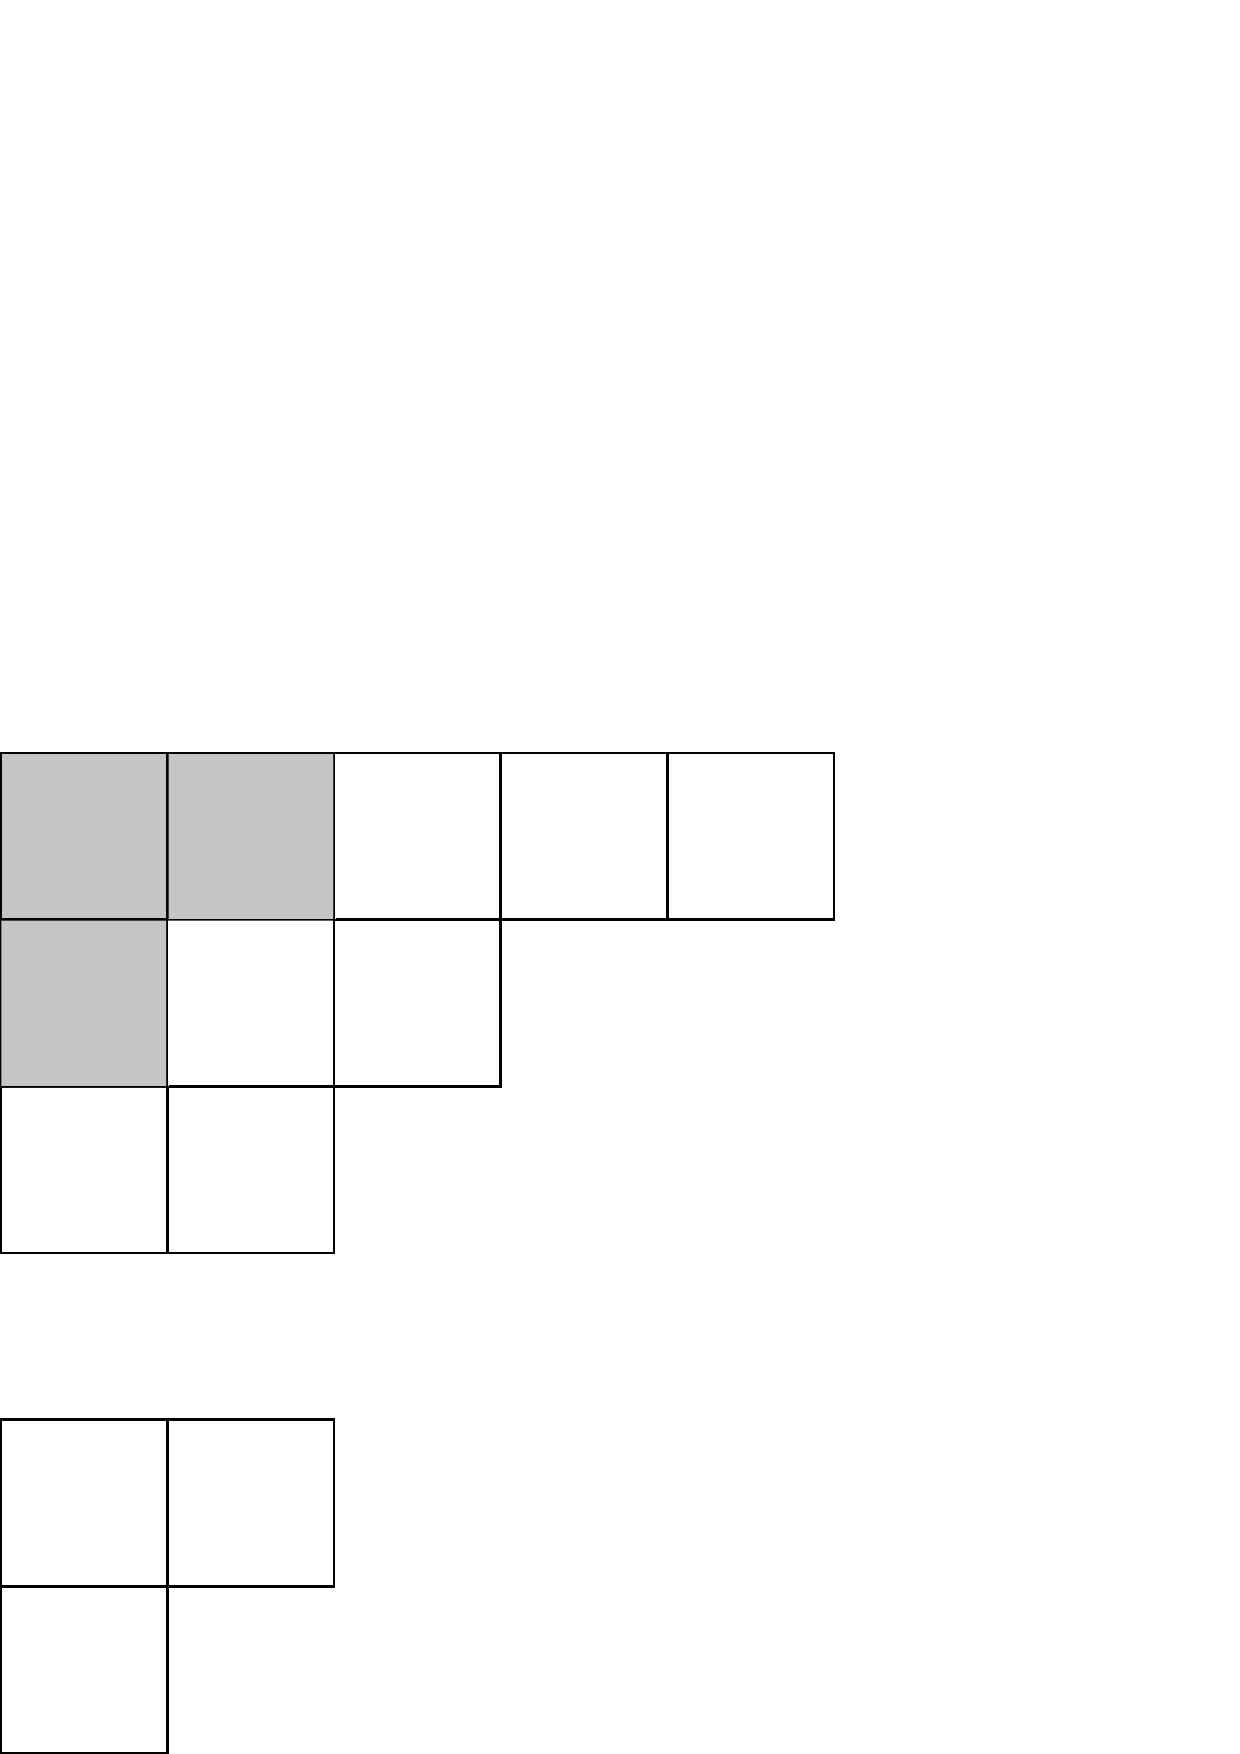
\includegraphics[width=0.7\textwidth]{images/skew_diag_2.pdf}\\
%% $\mu=(2,1)$
%% \end{column}
%% \begin{column}{3.3cm}
%% \includegraphics[width=0.7\textwidth]{images/skew_diag_3.pdf}\\
%% $\lambda / \mu$
%% \end{column}
%% \end{columns}
%% \end{frame}

\subsection{Young tableaux}

\begin{frame}
\frametitle{Young tableau}
\begin{columns}
\column{5cm}
\includegraphics[width=0.7\textwidth]{images/tableau.pdf}
\column{5cm}
\begin{enumerate}[(i)]
\item $T^i_j \leq T^i_{j+1}$
\item $T^i_j < T^{i+1}_j$
\end{enumerate}
\end{columns}
\end{frame}

\begin{frame}
\frametitle{Row bumping}
\centering
%% \begin{columns}[t]
%% \begin{column}{3.3cm}
%% \includegraphics[height=0.7\textwidth]{images/bump_1.pdf}\\
%% 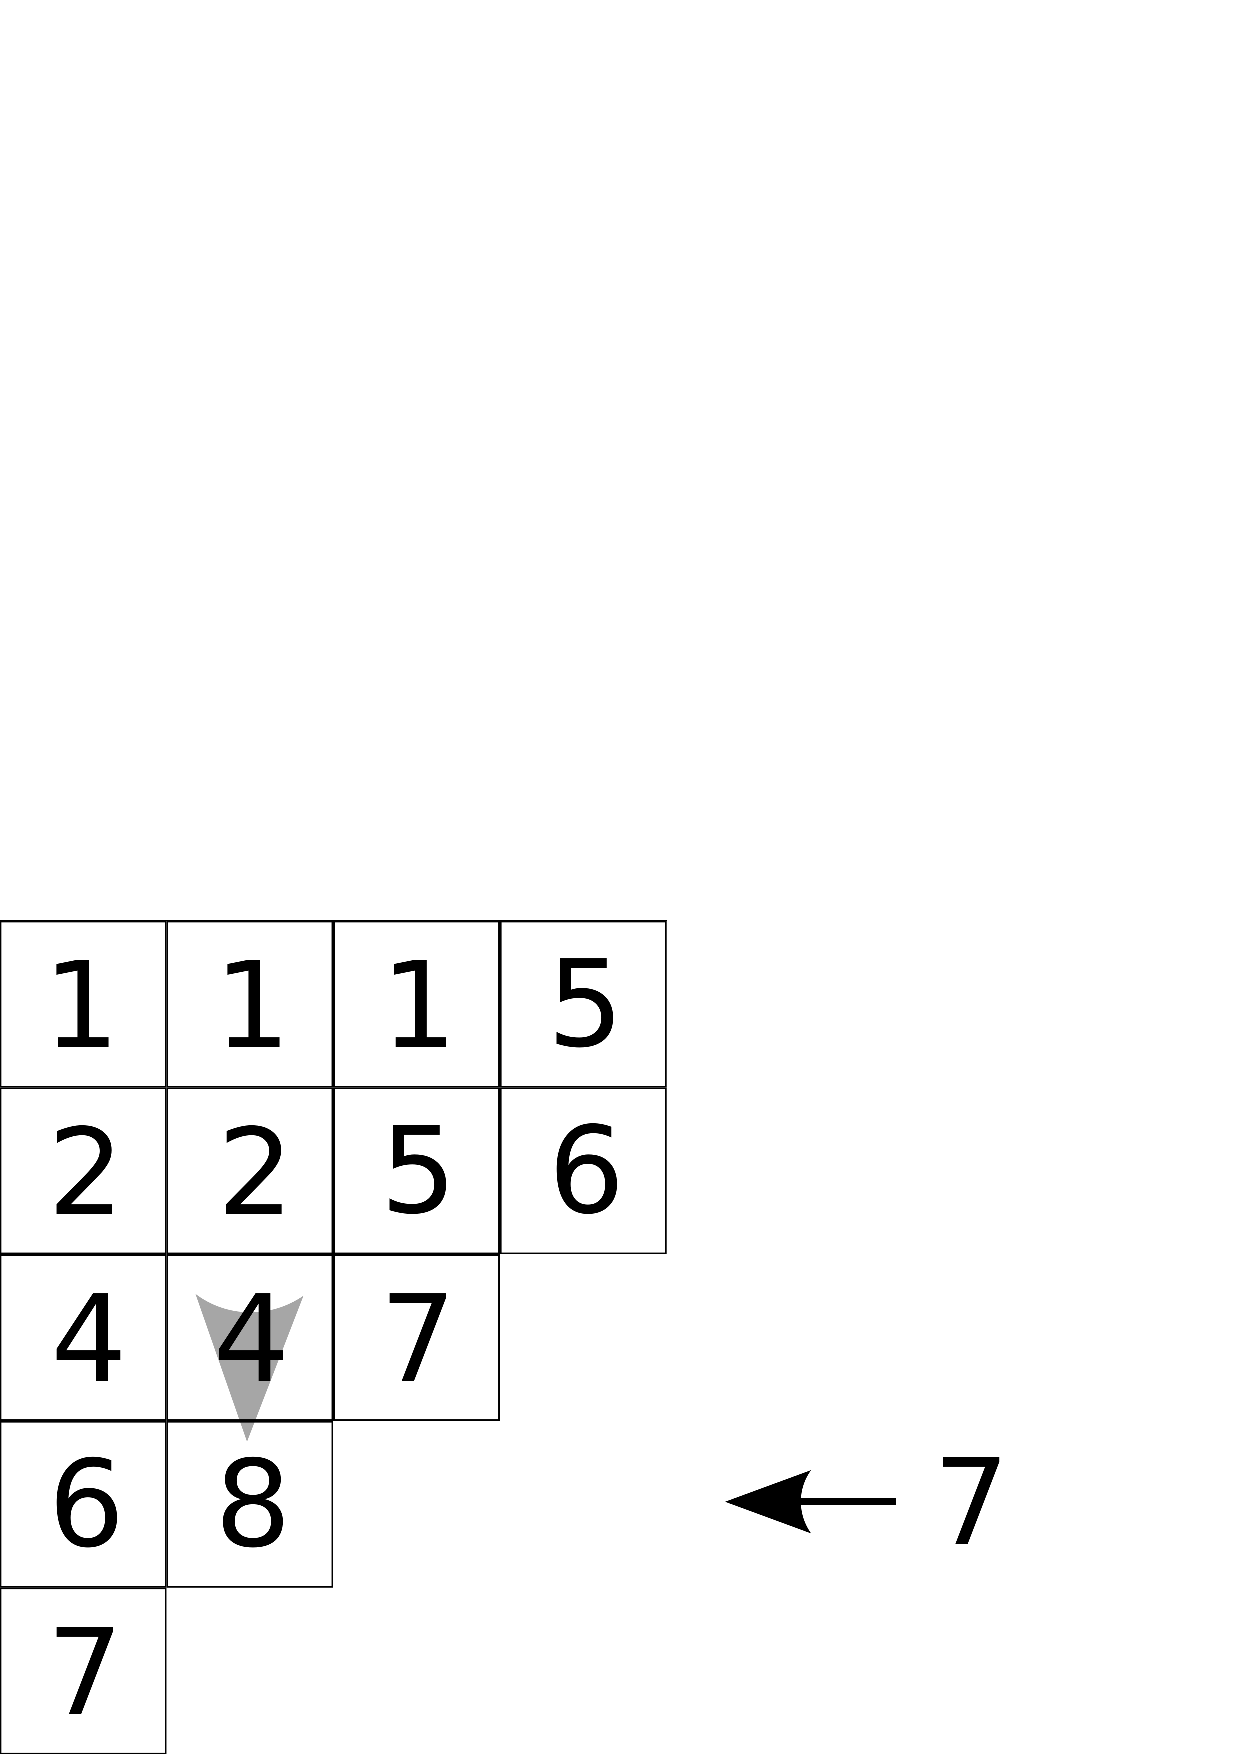
\includegraphics[height=0.6\textwidth]{images/bump_4.pdf}
%% \end{column}
%% \begin{column}{3.3cm}
%% 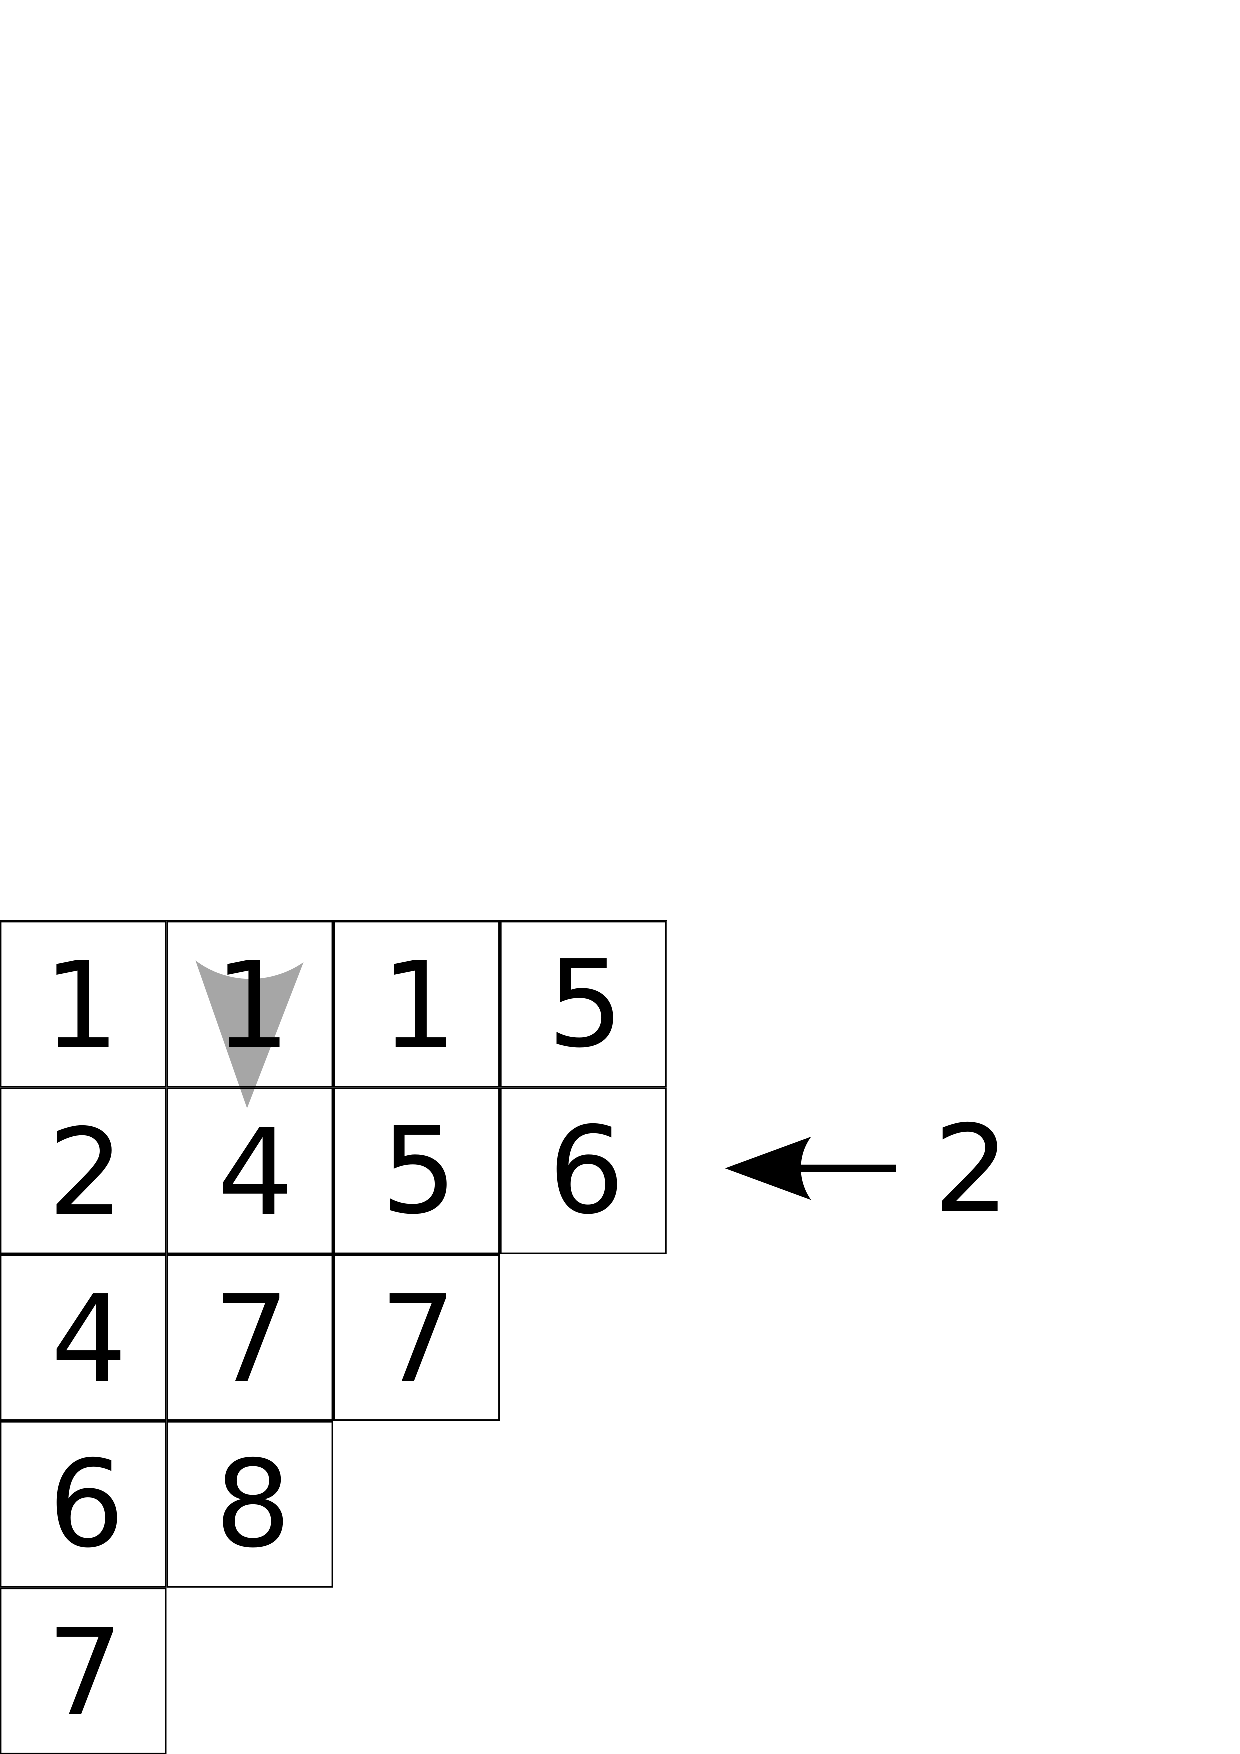
\includegraphics[height=0.6\textwidth]{images/bump_2.pdf}\\
%% \includegraphics[height=0.6\textwidth]{images/bump_5.pdf}
%% \end{column}
%% \begin{column}{3.3cm}
%% 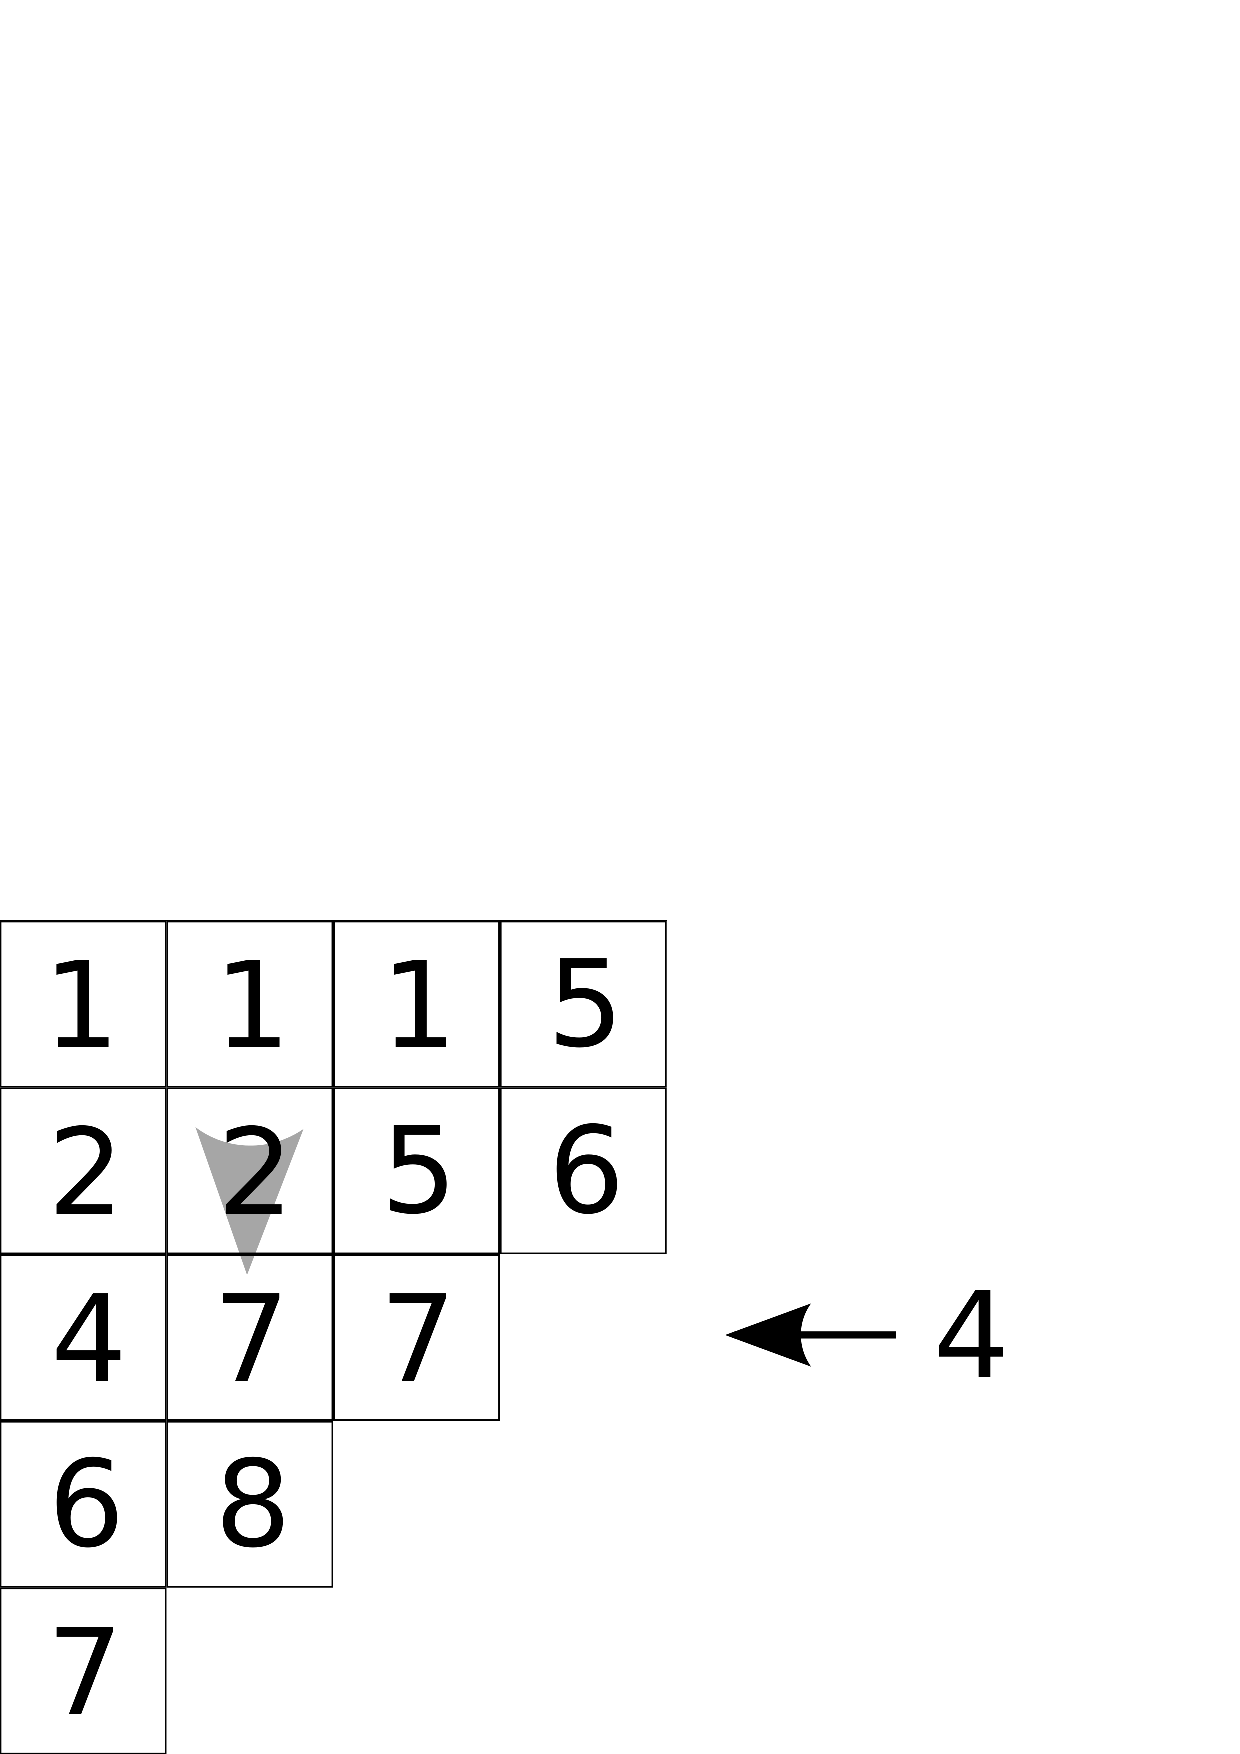
\includegraphics[height=0.6\textwidth]{images/bump_3.pdf}\\
%% 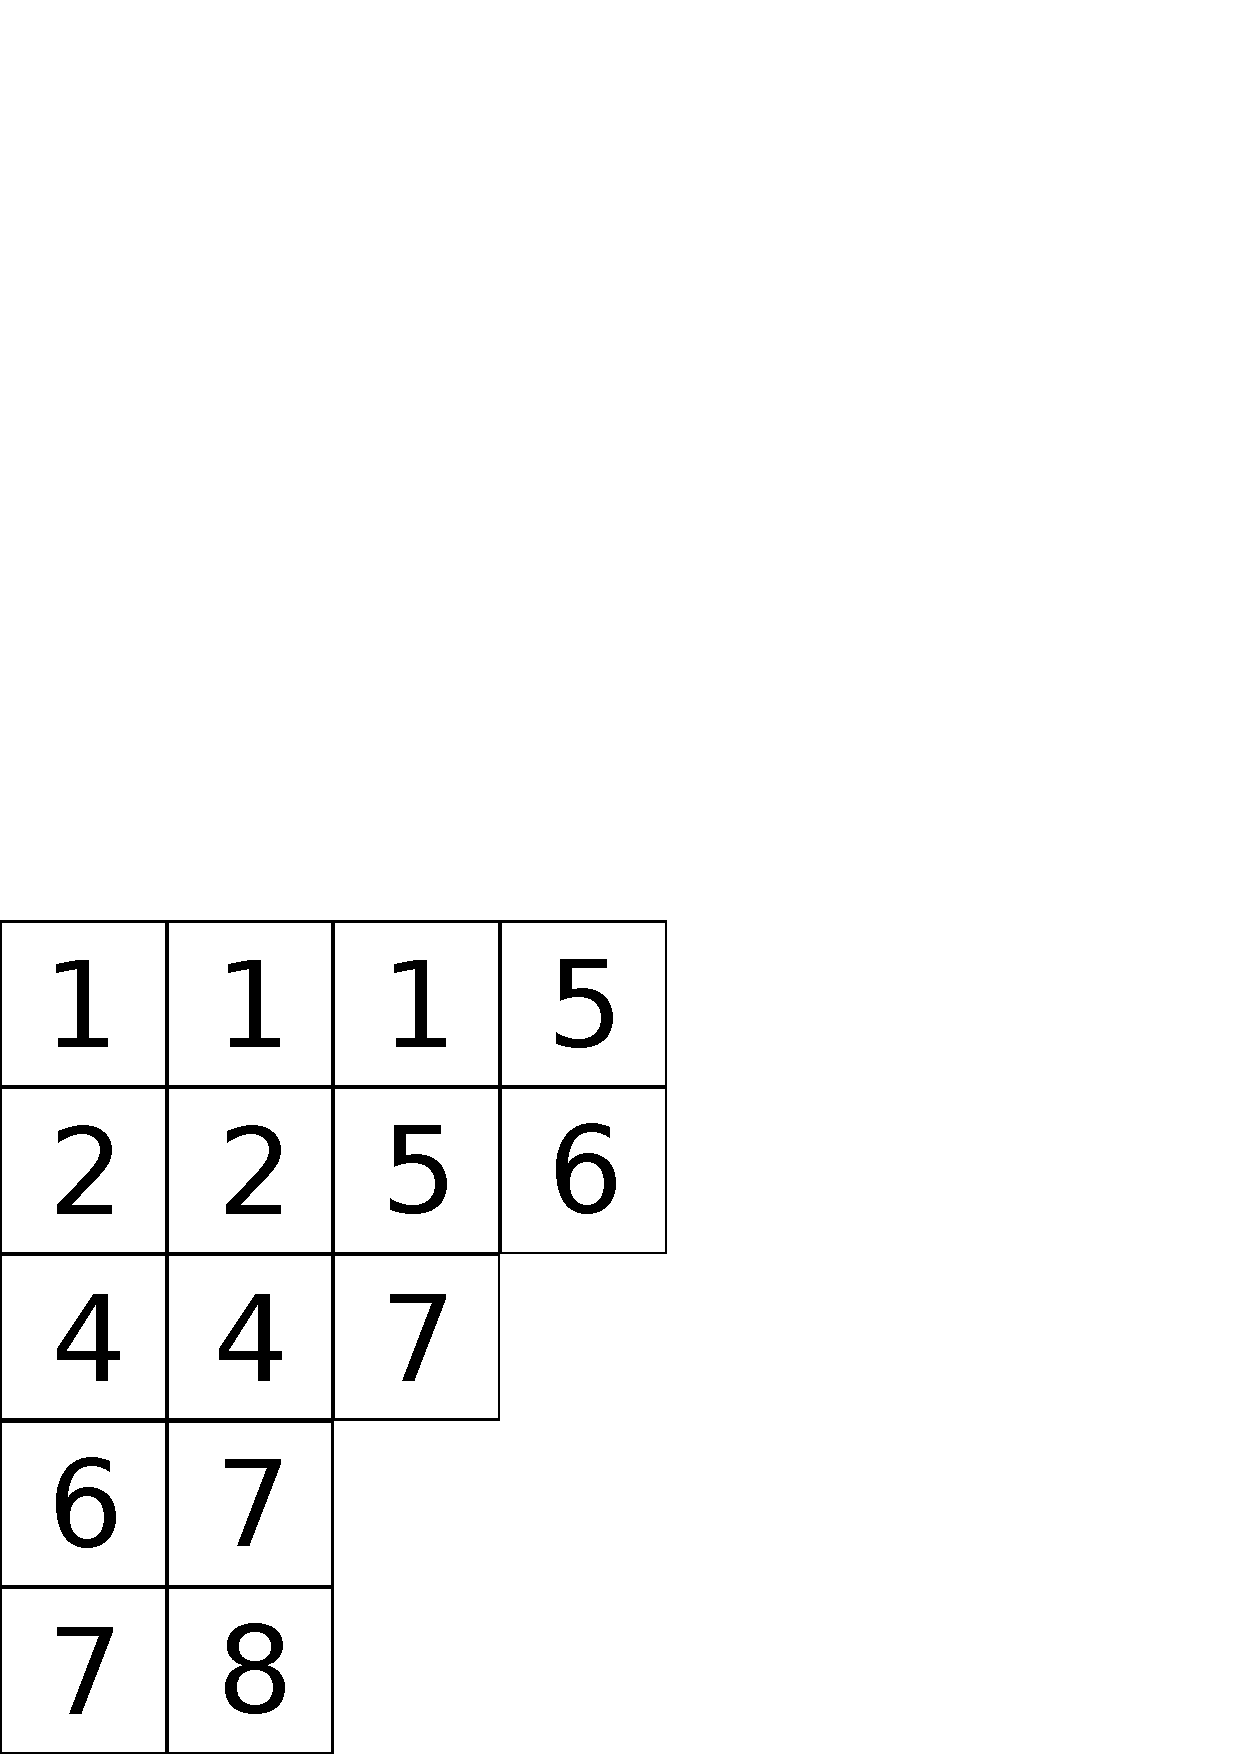
\includegraphics[height=0.6\textwidth]{images/bump_6.pdf}
%% \end{column}
%% \end{columns}
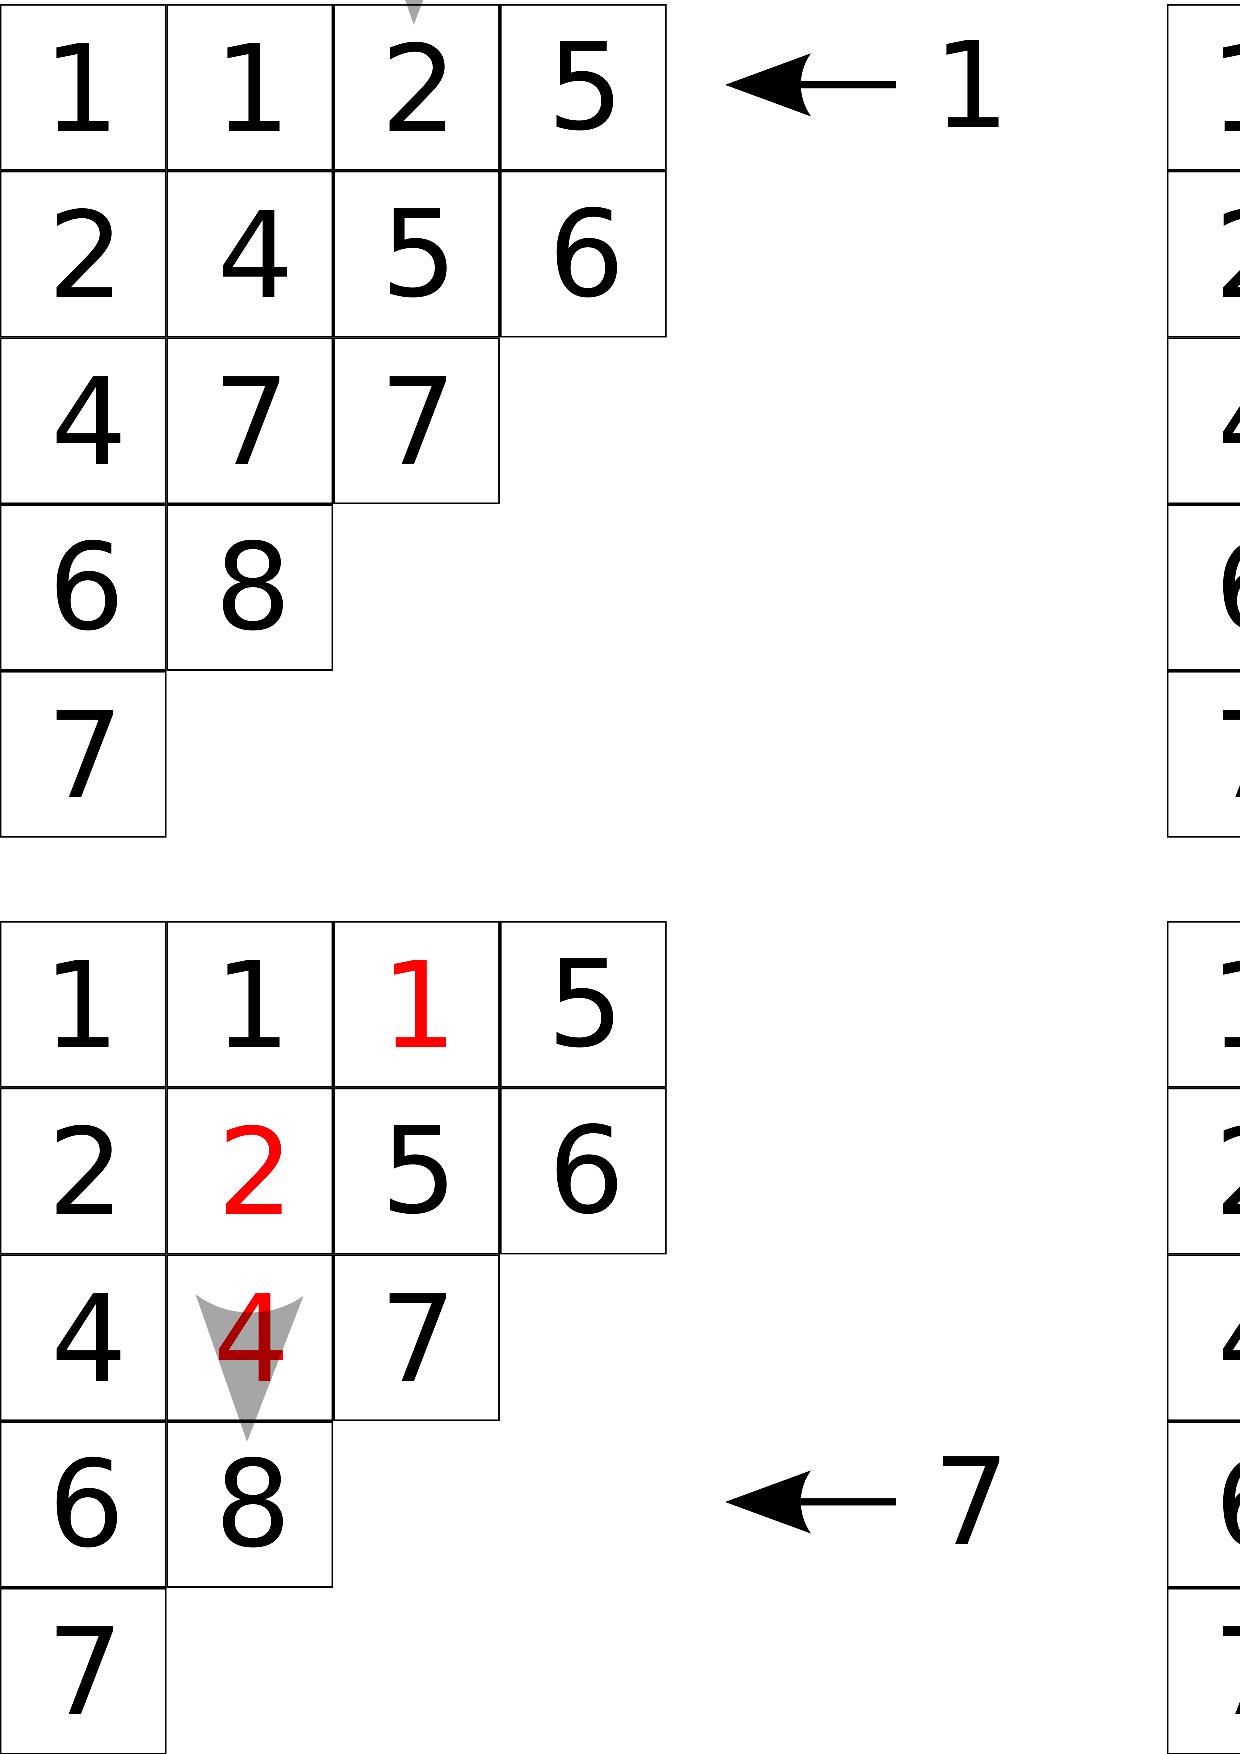
\includegraphics[width=\textwidth]{images/row_bump_slides.pdf}
\end{frame}

\begin{frame}
\frametitle{Prodotto di tableaux}
\centering
\begin{columns}[t]
\begin{column}{5cm}
\includegraphics[width=0.7\textwidth]{images/prod_1.pdf}
\vspace{1cm}
\includegraphics[width=0.6\textwidth]{images/prod_3_slides.pdf}
\end{column}
\begin{column}{5cm}
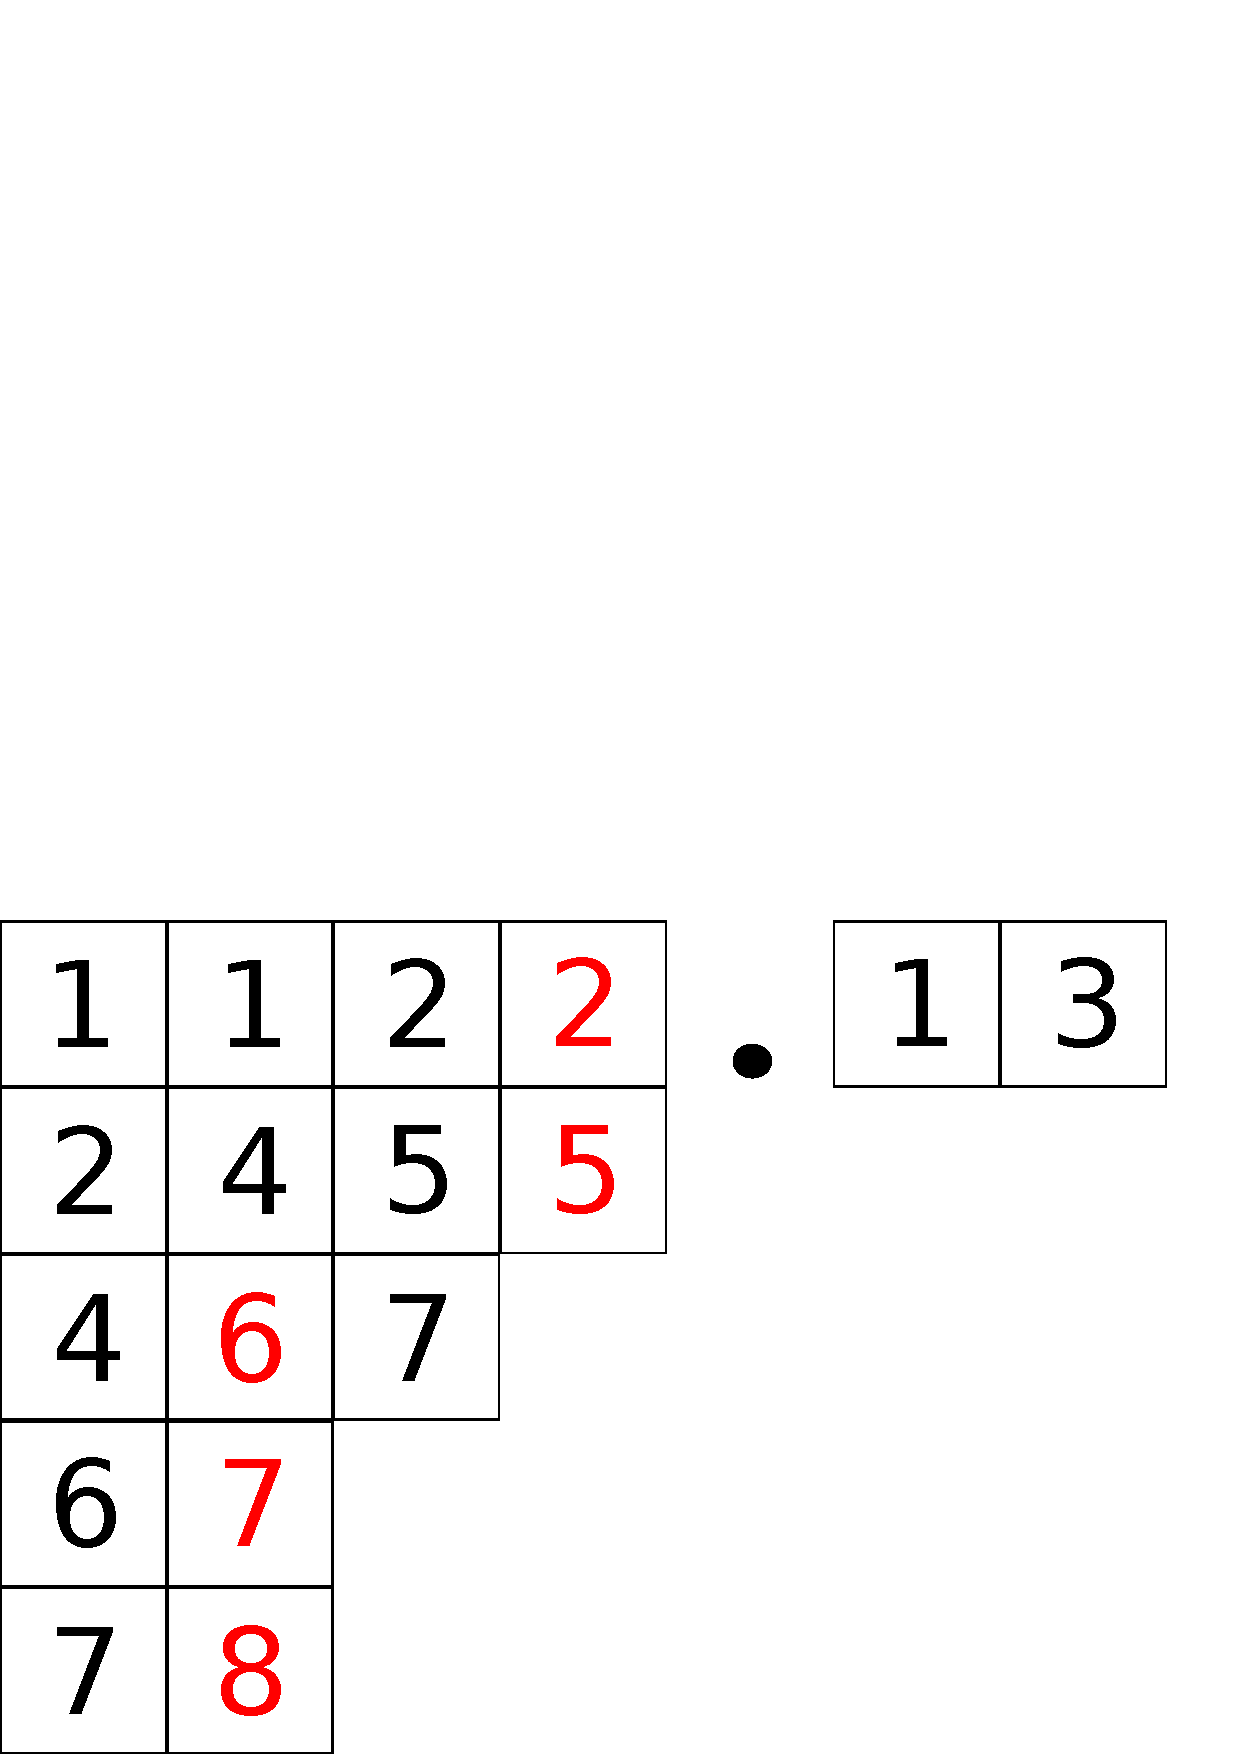
\includegraphics[width=0.7\textwidth]{images/prod_2_slides.pdf}
\vspace{1cm}
\includegraphics[width=0.5\textwidth]{images/prod_4_slides.pdf}
\end{column}
\end{columns}
\end{frame}

%% \subsection{Skew tableau}

\section{Polinomi di Schur}

\subsection{Definizione}

\begin{frame}
\frametitle{Monomio di un tableau}
\centering
\begin{columns}
\begin{column}{5cm}
%% \begin{overprint}
%% \onslide<2->
\includegraphics[width=0.4\textwidth]{images/tableau.pdf}
%% \end{overprint}
%% \begin{overprint}
%% \onslide<3->
\Large $x_1^2 x_2^2 x_4^2 x_5^2 x_6^2 x_7^3 x_8$
%% \end{overprint}
\end{column}
\begin{column}{5cm}
$x^T = \prod\limits_{i = 1}^m x_i^{c(i)}$\\
dove $c(i)=\#$ occorrenze \\\hspace{1cm} di $i$ nel tableau T
\end{column}
\end{columns}
\end{frame}

\begin{frame}
\frametitle{Polinomio di Schur}
$s_\lambda(x_1,\ldots,x_m) = \sum\limits_{T \text{ tableau su}\lambda}
x^T$
\vspace{1.5cm}
\begin{enumerate}[(i)]
\item i polinomi di Schur sono simmetrici
\item i polinomi di Schur di grado $n$ in $m$ indeterminate formano una
  base per i polinomi simmetrici omogenei di grado $n$ in $m$ indeterminate
\end{enumerate}
\end{frame}

\subsection{L'algoritmo}

\begin{frame}[t]
\frametitle{Polinomio di Schur}
\texttt{fl\_better\_yschur\_polynomial\_rows ([1,3,3], 3)}\\
$\rightarrow x_{1}\,x_{2}^3\,x_{3}^3+x_{1}^2\,x_{2}^2\,x_{3}^3+x_{1}^3\,x_{2}\,x
 _{3}^3+x_{1}^2\,x_{2}^3\,x_{3}^2+x_{1}^3\,x_{2}^2\,x_{3}^2+x_{1}^3\,
 x_{2}^3\,x_{3}$
\vspace{0.5cm}
\begin{overprint}[\textwidth]
\begin{columns}[T]
\begin{column}{5cm}
\begin{overprint}[\textwidth]
\onslide<2->
\centering
\includegraphics[height=0.2\textwidth]{images/yschur_1.pdf}
\end{overprint}
\end{column}
\begin{column}{5cm}
\begin{overprint}[\textwidth]
\centering
\onslide<3->
\includegraphics[height=0.2\textwidth]{images/yschur_2.pdf}
\end{overprint}
\end{column}
\end{columns}
\vspace{0.5cm}
\begin{columns}[T]
\begin{column}{3.33cm}
\centering
\includegraphics<4->[height=0.3\textwidth]{images/yschur_3.pdf}
\end{column}
\begin{column}{3.33cm}
\centering
\includegraphics<4>[height=0.3\textwidth]{images/yschur_4.pdf}
\includegraphics<5->[height=0.3\textwidth]{images/yschur_6.pdf}
\end{column}
\begin{column}{3.33cm}
\centering
\includegraphics<4>[height=0.3\textwidth]{images/yschur_5.pdf}
\includegraphics<5->[height=0.3\textwidth]{images/yschur_7.pdf}
\end{column}
\end{columns}
\vspace{0.5cm}
\begin{overprint}[\textwidth]
\onslide<6->
\begin{columns}[c]
\column{3.33cm}
\centering
\includegraphics[height=0.3\textwidth]{images/yschur_8.pdf}
\column{3.33cm}
\centering
\includegraphics[height=0.3\textwidth]{images/yschur_9.pdf}
\column{3.33cm}
\centering
\includegraphics[height=0.3\textwidth]{images/yschur_10.pdf}
\end{columns}
\end{overprint}
\end{overprint}
\end{frame}

%% \begin{columns}[T]
%% \begin{column}{5cm}
%% \includegraphics[width=\textwidth]{images/schur_poly_demo.png}
%% \end{column}
%% \begin{column}{5cm}

%% \begin{columns}[T]
%% \begin{column}{2.5cm}
%% \begin{overprint}[\textwidth]
%% \onslide<2->
%% \includegraphics[height=0.4\textwidth]{images/yschur_1.pdf}
%% \end{overprint}
%% \end{column}
%% \begin{column}{2.5cm}
%% \begin{overprint}[\textwidth]
%% \onslide<3->
%% \includegraphics[height=0.4\textwidth]{images/yschur_2.pdf}
%% \end{overprint}
%% \end{column}
%% \end{columns}

%% \begin{overprint}[\textwidth]
%% \begin{columns}[b]
%% \column{1.66cm}
%% \includegraphics<4->[height=0.6\textwidth]{images/yschur_3.pdf}
%% \column{1.66cm}
%% \includegraphics<4>[height=0.6\textwidth]{images/yschur_4.pdf}
%% \includegraphics<5->[height=0.6\textwidth]{images/yschur_6.pdf}
%% \column{1.66cm}
%% \includegraphics<4>[height=0.6\textwidth]{images/yschur_5.pdf}
%% \includegraphics<5->[height=0.6\textwidth]{images/yschur_7.pdf}
%% \end{columns}
%% \end{overprint}

%% \begin{overprint}[\textwidth]
%% \onslide<6->
%% \begin{columns}[c]
%% \column{1.66cm}
%% \includegraphics[height=0.6\textwidth]{images/yschur_8.pdf}
%% \column{1.66cm}
%% \includegraphics[height=0.6\textwidth]{images/yschur_9.pdf}
%% \column{1.66cm}
%% \includegraphics[height=0.6\textwidth]{images/yschur_10.pdf}
%% \end{columns}
%% \end{overprint}

%% \end{column}
%% \end{columns}
%% \end{frame}

\begin{frame}
\frametitle{Polinomio di Schur}
\begin{columns}[c]
\column{3.33cm}
%% \includegraphics<1>[height=0.7\textwidth]{images/yschur_11.pdf}\\
%% \includegraphics<1>[height=0.7\textwidth]{images/yschur_12.pdf}
\includegraphics[height=0.5\textwidth]{images/yschur_11.pdf}
\vspace{0.5cm}
\includegraphics[height=0.5\textwidth]{images/yschur_12.pdf}
\column{3.33cm}
%% \includegraphics<1>[height=0.7\textwidth]{images/yschur_13.pdf}\\
%% \includegraphics<1>[height=0.7\textwidth]{images/yschur_14.pdf}
\includegraphics[height=0.5\textwidth]{images/yschur_13.pdf}
\vspace{0.5cm}
\includegraphics[height=0.5\textwidth]{images/yschur_14.pdf}
\column{3.33cm}
%% \includegraphics<1>[height=0.7\textwidth]{images/yschur_15.pdf}\\
%% \includegraphics<1>[height=0.7\textwidth]{images/yschur_16.pdf}
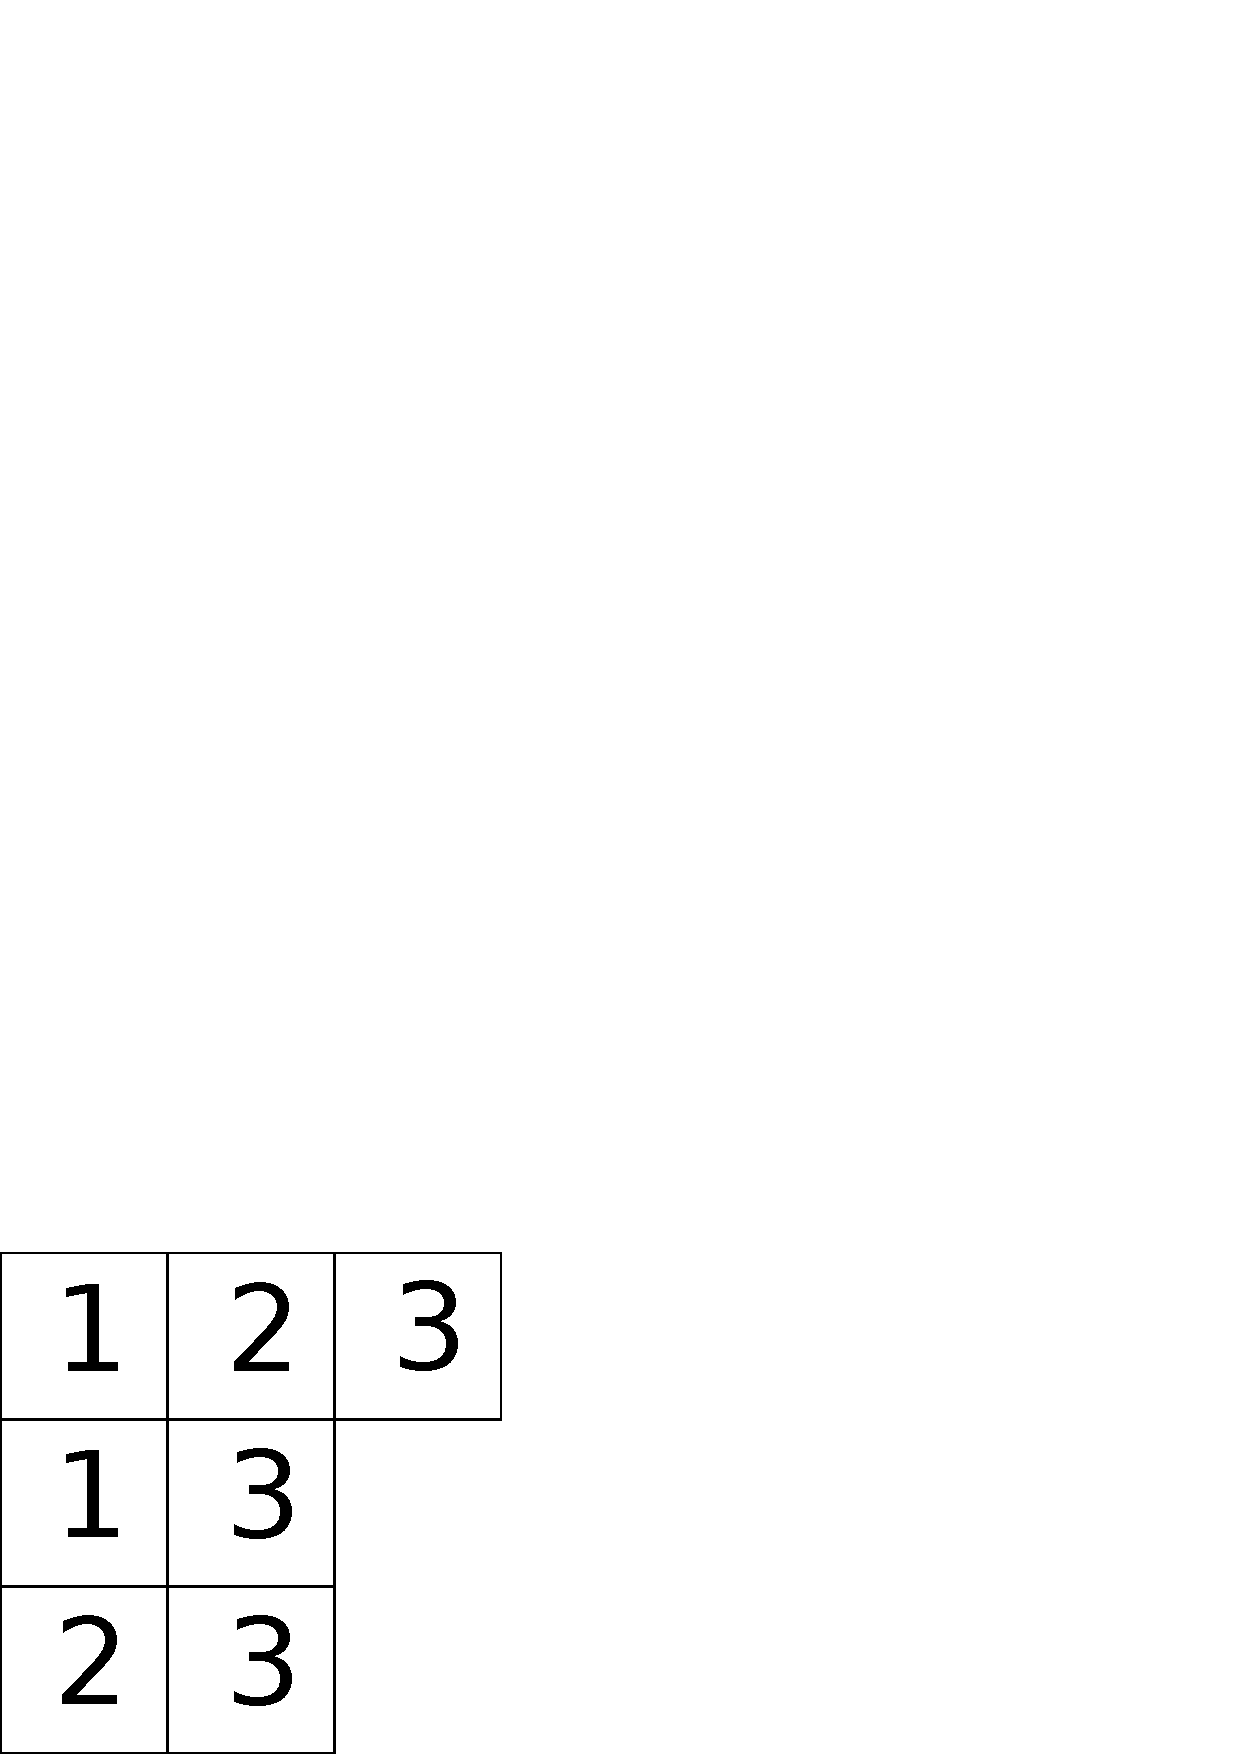
\includegraphics[height=0.5\textwidth]{images/yschur_15.pdf}
\vspace{0.5cm}
\includegraphics[height=0.5\textwidth]{images/yschur_16.pdf}
\end{columns}
\vspace{0.5cm}
\Large$s_{(1,3,3)}(x_1,x_2,x_3)=x_{1}\,x_{2}^3\,x_{3}^3+x_{1}^2\,x_{2}^2\,x_{3}^3+x_{1}^3\,x_{2}\,x_{3}^3+x_{1}^2\,x_{2}^3\,x_{3}^2+x_{1}^3\,x_{2}^2\,x_{3}^2+x_{1}^3\,x_{2}^3\,x_{3}$
\end{frame}

\section{Littlewood-Richardson}

\subsection{I numeri di Littlewood-Richardson}

\begin{frame}
\frametitle{``Contare'' i prodotti di tabelle}
\begin{block}{}
$s_{\lambda}(x_1,\ldots,x_m) \cdot s_{\mu}(x_1,\ldots,x_m) =
\sum\limits_{\nu} c_{\lambda \mu}^{\nu} s_{\nu}(x_1,\ldots,x_m)$\\
dove $c_{\lambda \mu}^\nu=card\left(\{ (T,U) \mid V = T \cdot U; T,U \text{
  tableaux su } \lambda \text{ e } \mu \text{ risp.}\}\right)$
\end{block}
\vspace{1cm}
\begin{block}{Problema}
Metodo per calcolare i numeri di Littlewood-Richardson.
\end{block}
\end{frame}

\subsection{L'algoritmo}

\begin{frame}
\frametitle{Skew tableaux di Littlewood-Richardson}
\begin{columns}[T]
\column{5cm}
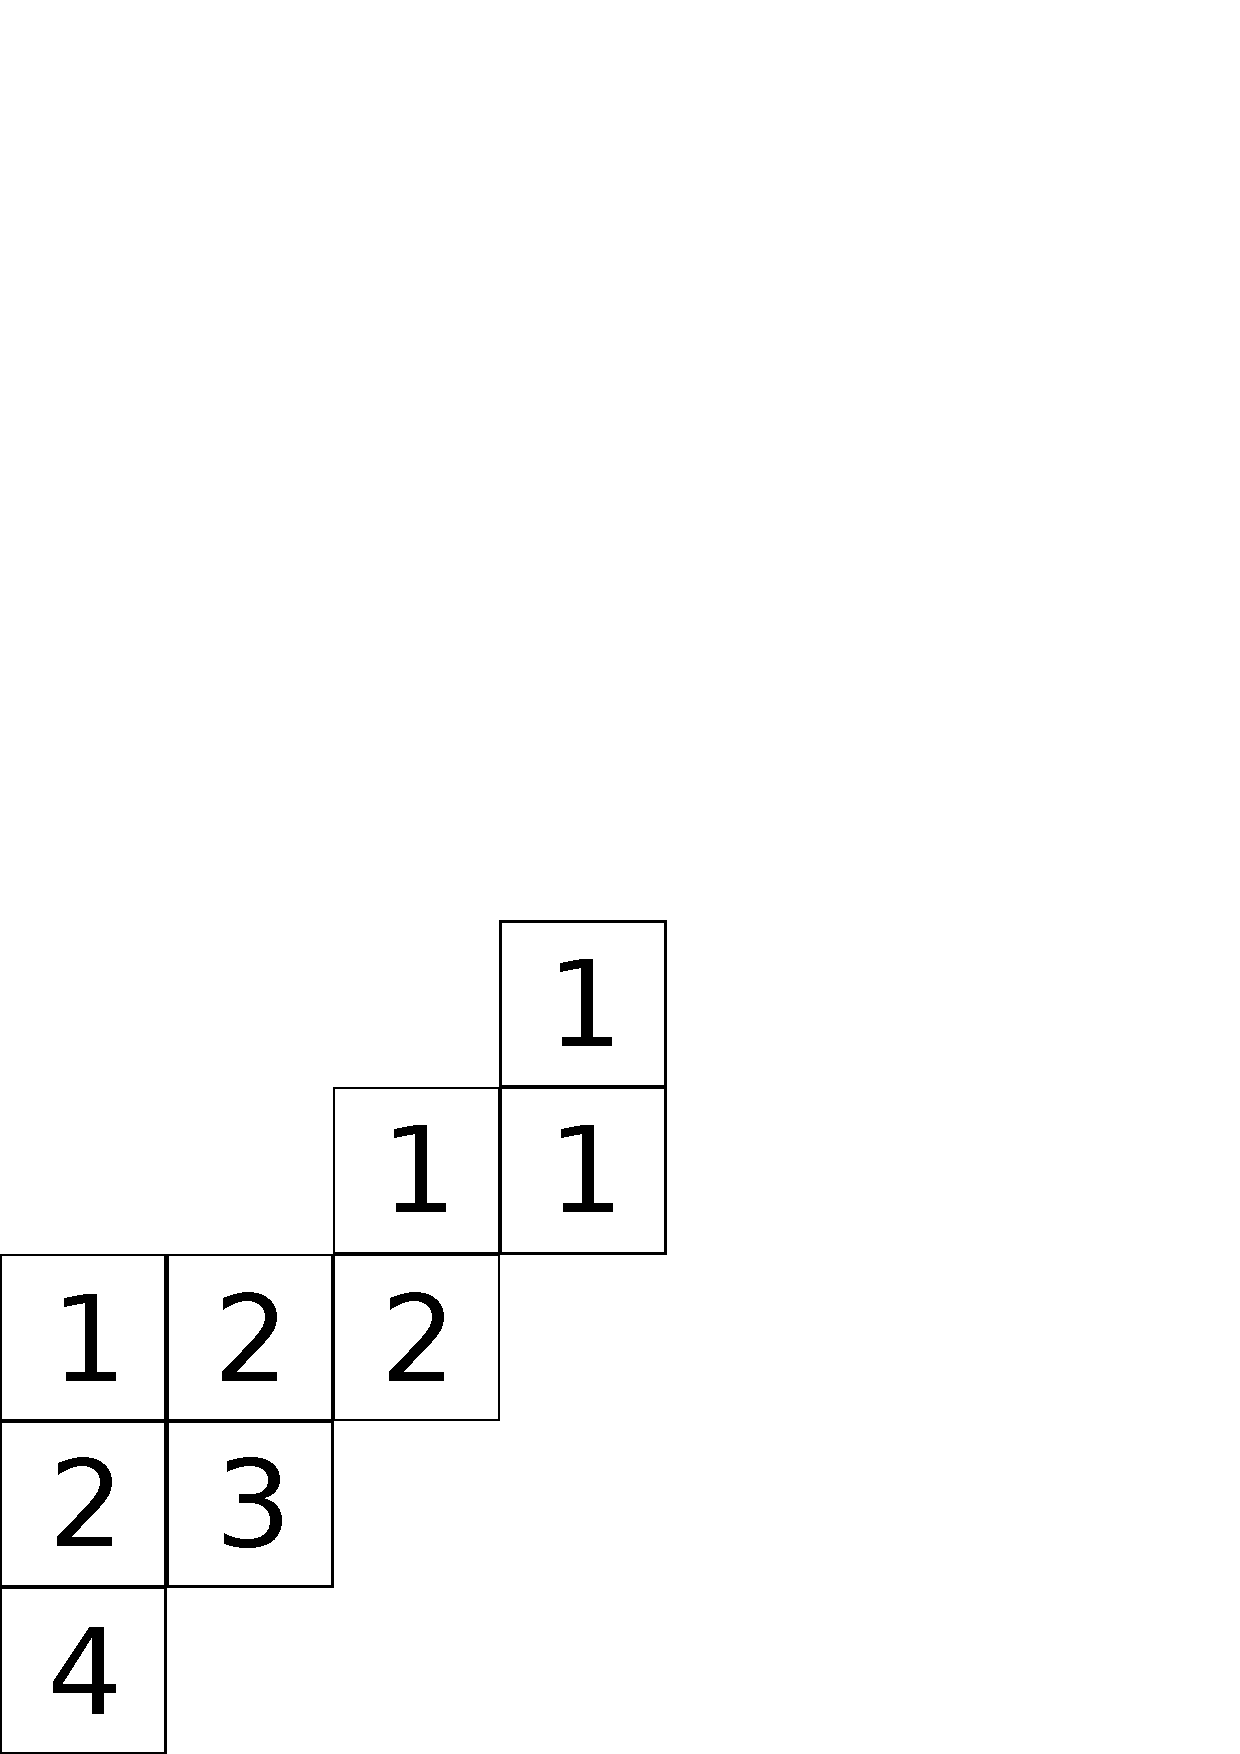
\includegraphics[width=0.8\textwidth]{images/littlewood-richardson_skew_tableau.pdf}
\column{5cm}
\begin{enumerate}[(i)]
\item skew tableau $T$
\item $w(T)$ reverse lattice word
\end{enumerate}
\vspace{1cm}
skew tableau su $\nu / \lambda = (4,4,3,2,1) / (3,2)$\\
\emph{contenuto} $\mu=(3,3,1,1)$
\end{columns}
\end{frame}

\begin{frame}
\frametitle{Calcolo dei numeri di Littlewood-Richardson}
\begin{block}{Proposizione}
Il numero di skew tableaux di Littlewood-Richardson che riempiono lo
skew diagram $\nu/\lambda$ con contenuto $\mu$ \`e $c_{\lambda \mu}^{\nu}$.
\end{block}
\begin{block}{Un esempio}
\begin{enumerate}[(i)]
\item $\lambda=(1,2,3), \mu=(1,3,3)$
\item $\nu$ diagramma di Young costruito a partire da $\lambda$
\item numero di skew tableaux di Littlewood-Richardson su $\nu /
  \lambda$ con contenuto $\mu$
\end{enumerate} 
\end{block}
\end{frame}

\begin{frame}[t]
\frametitle{Verifica}
\tiny
\begin{align*}
\texttt{lr\_calc([3,2,1],[3,3,1]);}\rightarrow
&[[3,3,3,2,1,1],1],[[3,3,3,2,2],1],[[3,3,3,3,1],1],[[4,3,2,2,1,1],1],[[4,3,2,2,2],1],\\
&[[4,3,3,1,1,1],1],[[4,3,3,2,1],3],[[4,3,3,3],1],[[4,4,2,1,1,1],1],[[4,4,2,2,1],2],\\
&[[4,4,3,1,1],2],[[4,4,3,2],2],[[4,4,4,1],1],[[5,3,2,1,1,1],1],[[5,3,2,2,1],2],\\
&[[5,3,3,1,1],2],[[5,3,3,2],2],[[5,4,1,1,1,1],1],[[5,4,2,1,1],3],[[5,4,2,2],2],\\
&[[5,4,3,1],3],[[5,4,4],1],[[5,5,1,1,1],1],[[5,5,2,1],2],[[5,5,3],1],[[6,3,2,1,1],1],\\
&[[6,3,2,2],1],[[6,3,3,1],1],[[6,4,1,1,1],1],[[6,4,2,1],2],[[6,4,3],1],[[6,5,1,1],1],\\
&[[6,5,2],1]
\end{align*}
\begin{align*}
&s_{(1,2,3)}(x_1,x_2,x_3,x_4)\cdot s_{(1,3,3)}(x_1,x_2,x_3,x_4)=\\
&=s_{(3,3,3,2,1,1)}(x_1,x_2,x_3,x_4)+s_{(3,3,3,2,2)}(x_1,x_2,x_3,x_4)+s_{(3,3,3,3,1)}(x_1,x_2,x_3,x_4)+s_{(4,3,2,2,1,1)}(x_1,x_2,x_3,x_4)+\\
&+s_{(4,3,2,2,2)}(x_1,x_2,x_3,x_4)+s_{(4,3,3,1,1,1)}(x_1,x_2,x_3,x_4)+3s_{(4,3,3,2,1)}(x_1,x_2,x_3,x_4)+s_{(4,3,3,3)}(x_1,x_2,x_3,x_4)+\\
&+s_{(4,4,2,1,1,1)}(x_1,x_2,x_3,x_4)+2s_{(4,4,2,2,1)}(x_1,x_2,x_3,x_4)+2s_{(4,4,3,1,1)}(x_1,x_2,x_3,x_4)+2s_{(4,4,3,2)}(x_1,x_2,x_3,x_4)+\\
&+s_{(4,4,4,1)}(x_1,x_2,x_3,x_4)+s_{(5,3,2,1,1,1)}(x_1,x_2,x_3,x_4)+2s_{(5,3,2,2,1)}(x_1,x_2,x_3,x_4)+2s_{(5,3,3,1,1)}(x_1,x_2,x_3,x_4)+\\
&+2s_{(5,3,3,2)}(x_1,x_2,x_3,x_4)+s_{(5,4,1,1,1,1)}(x_1,x_2,x_3,x_4)+3s_{(5,4,2,1,1)}(x_1,x_2,x_3,x_4)+2s_{(5,4,2,2)}(x_1,x_2,x_3,x_4)+\\
&+3s_{(5,4,3,1)}(x_1,x_2,x_3,x_4)+s_{(5,4,4)}(x_1,x_2,x_3,x_4)+s_{(5,5,1,1,1)}(x_1,x_2,x_3,x_4)+2s_{(5,5,2,1)}(x_1,x_2,x_3,x_4)+\\
&+s_{(5,5,3)}(x_1,x_2,x_3,x_4)+s_{(6,3,2,1,1)}(x_1,x_2,x_3,x_4)+s_{(6,3,2,2)}(x_1,x_2,x_3,x_4)+s_{(6,3,3,1)}(x_1,x_2,x_3,x_4)+\\
&+s_{(6,4,1,1,1)}(x_1,x_2,x_3,x_4)+2s_{(6,4,2,1)}(x_1,x_2,x_3,x_4)+s_{(6,4,3)}(x_1,x_2,x_3,x_4)+s_{(6,5,1,1)}(x_1,x_2,x_3,x_4)+\\
&+s_{(6,5,2)}(x_1,x_2,x_3,x_4).
\end{align*}

\end{frame}

%% \begin{frame}[t]
%% \frametitle{Verifica}
%% \only<1>{\textcolor{blue}{$s_{(1,2,3)}(x_1,x_2,x_3,x_4)$}$\cdot s_{(1,3,3)}(x_1,x_2,x_3,x_4)$}
%% \only<2>{$s_{(1,2,3)}(x_1,x_2,x_3,x_4)\cdot$\textcolor{blue}{$s_{(1,3,3)}(x_1,x_2,x_3,x_4)$}}
%% \only<1>{\textcolor{blue}{\texttt{fl\_better\_yschur\_polynomial\_rows([1,2,3],4);}}}
%% \only<2>{\textcolor{blue}{\texttt{fl\_better\_yschur\_polynomial\_rows([1,3,3],4);}}}
%% \small
%% \only<1>{\begin{align*}
%% &\rightarrow
%%   {x}_{2}\,{x}_{3}^{2}\,{x}_{4}^{3}+{x}_{1}\,{x}_{3}^{2}\,{x}_{4}^{3}+{x}_{2}^{2}\,{x}_{3}\,{x}_{4}^{3}+2\,{x}_{1}\,{x}_{2}\,{x}_{3}\,{x}_{4}^{3}+{x}_{1}^{2}\,{x}_{3}\,{x}_{4}^{3}+{x}_{1}\,{x}_{2}^{2}\,{x}_{4}^{3}+{x}_{1}^{2}\,{x}_{2}\,{x}_{4}^{3}+\\
%% &+{x}_{2}\,{x}_{3}^{3}\,{x}_{4}^{2}+{x}_{1}\,{x}_{3}^{3}\,{x}_{4}^{2}+2\,{x}_{2}^{2}\,{x}_{3}^{2}\,{x}_{4}^{2}+4\,{x}_{1}\,{x}_{2}\,{x}_{3}^{2}\,{x}_{4}^{2}+2\,{x}_{1}^{2}\,{x}_{3}^{2}\,{x}_{4}^{2}+{x}_{2}^{3}\,{x}_{3}\,{x}_{4}^{2}+\\
%% &+4\,{x}_{1}\,{x}_{2}^{2}\,{x}_{3}\,{x}_{4}^{2}+4\,{x}_{1}^{2}\,{x}_{2}\,{x}_{3}\,{x}_{4}^{2}+{x}_{1}^{3}\,{x}_{3}\,{x}_{4}^{2}+{x}_{1}\,{x}_{2}^{3}\,{x}_{4}^{2}+2\,{x}_{1}^{2}\,{x}_{2}^{2}\,{x}_{4}^{2}+{x}_{1}^{3}\,{x}_{2}\,{x}_{4}^{2}+\\
%% &+{x}_{2}^{2}\,{x}_{3}^{3}\,{x}_{4}+2\,{x}_{1}\,{x}_{2}\,{x}_{3}^{3}\,{x}_{4}+{x}_{1}^{2}\,{x}_{3}^{3}\,{x}_{4}+{x}_{2}^{3}\,{x}_{3}^{2}\,{x}_{4}+4\,{x}_{1}\,{x}_{2}^{2}\,{x}_{3}^{2}\,{x}_{4}+\\
%% &+4\,{x}_{1}^{2}\,{x}_{2}\,{x}_{3}^{2}\,{x}_{4}+{x}_{1}^{3}\,{x}_{3}^{2}\,{x}_{4}+2\,{x}_{1}\,{x}_{2}^{3}\,{x}_{3}\,{x}_{4}+4\,{x}_{1}^{2}\,{x}_{2}^{2}\,{x}_{3}\,{x}_{4}+2\,{x}_{1}^{3}\,{x}_{2}\,{x}_{3}\,{x}_{4}+\\
%% &+{x}_{1}^{2}\,{x}_{2}^{3}\,{x}_{4}+{x}_{1}^{3}\,{x}_{2}^{2}\,{x}_{4}+{x}_{1}\,{x}_{2}^{2}\,{x}_{3}^{3}+{x}_{1}^{2}\,{x}_{2}\,{x}_{3}^{3}+{x}_{1}\,{x}_{2}^{3}\,{x}_{3}^{2}+2\,{x}_{1}^{2}\,{x}_{2}^{2}\,{x}_{3}^{2}+\\
%% &+{x}_{1}^{3}\,{x}_{2}\,{x}_{3}^{2}+{x}_{1}^{2}\,{x}_{2}^{3}\,{x}_{3}+{x}_{1}^{3}\,{x}_{2}^{2}\,{x}_{3}
%% \end{align*}}
%% \only<2>{\begin{align*}
%% &\rightarrow
%%   {x}_{2}\,{x}_{3}^{3}\,{x}_{4}^{3}+{x}_{1}\,{x}_{3}^{3}\,{x}_{4}^{3}+{x}_{2}^{2}\,{x}_{3}^{2}\,{x}_{4}^{3}+2\,{x}_{1}\,{x}_{2}\,{x}_{3}^{2}\,{x}_{4}^{3}+{x}_{1}^{2}\,{x}_{3}^{2}\,{x}_{4}^{3}+{x}_{2}^{3}\,{x}_{3}\,{x}_{4}^{3}+\\
%% &+2\,{x}_{1}\,{x}_{2}^{2}\,{x}_{3}\,{x}_{4}^{3}+2\,{x}_{1}^{2}\,{x}_{2}\,{x}_{3}\,{x}_{4}^{3}+{x}_{1}^{3}\,{x}_{3}\,{x}_{4}^{3}+{x}_{1}\,{x}_{2}^{3}\,{x}_{4}^{3}+{x}_{1}^{2}\,{x}_{2}^{2}\,{x}_{4}^{3}+{x}_{1}^{3}\,{x}_{2}\,{x}_{4}^{3}+\\
%% &+{x}_{2}^{2}\,{x}_{3}^{3}\,{x}_{4}^{2}+2\,{x}_{1}\,{x}_{2}\,{x}_{3}^{3}\,{x}_{4}^{2}+{x}_{1}^{2}\,{x}_{3}^{3}\,{x}_{4}^{2}+{x}_{2}^{3}\,{x}_{3}^{2}\,{x}_{4}^{2}+3\,{x}_{1}\,{x}_{2}^{2}\,{x}_{3}^{2}\,{x}_{4}^{2}+3\,{x}_{1}^{2}\,{x}_{2}\,{x}_{3}^{2}\,{x}_{4}^{2}+\\
%% &+{x}_{1}^{3}\,{x}_{3}^{2}\,{x}_{4}^{2}+2\,{x}_{1}\,{x}_{2}^{3}\,{x}_{3}\,{x}_{4}^{2}+3\,{x}_{1}^{2}\,{x}_{2}^{2}\,{x}_{3}\,{x}_{4}^{2}+2\,{x}_{1}^{3}\,{x}_{2}\,{x}_{3}\,{x}_{4}^{2}+{x}_{1}^{2}\,{x}_{2}^{3}\,{x}_{4}^{2}+{x}_{1}^{3}\,{x}_{2}^{2}\,{x}_{4}^{2}+\\
%% &+{x}_{2}^{3}\,{x}_{3}^{3}\,{x}_{4}+2\,{x}_{1}\,{x}_{2}^{2}\,{x}_{3}^{3}\,{x}_{4}+2\,{x}_{1}^{2}\,{x}_{2}\,{x}_{3}^{3}\,{x}_{4}+{x}_{1}^{3}\,{x}_{3}^{3}\,{x}_{4}+2\,{x}_{1}\,{x}_{2}^{3}\,{x}_{3}^{2}\,{x}_{4}+3\,{x}_{1}^{2}\,{x}_{2}^{2}\,{x}_{3}^{2}\,{x}_{4}+\\
%% &+2\,{x}_{1}^{3}\,{x}_{2}\,{x}_{3}^{2}\,{x}_{4}+2\,{x}_{1}^{2}\,{x}_{2}^{3}\,{x}_{3}\,{x}_{4}+2\,{x}_{1}^{3}\,{x}_{2}^{2}\,{x}_{3}\,{x}_{4}+{x}_{1}^{3}\,{x}_{2}^{3}\,{x}_{4}+{x}_{1}\,{x}_{2}^{3}\,{x}_{3}^{3}+{x}_{1}^{2}\,{x}_{2}^{2}\,{x}_{3}^{3}+\\
%% &+{x}_{1}^{3}\,{x}_{2}\,{x}_{3}^{3}+{x}_{1}^{2}\,{x}_{2}^{3}\,{x}_{3}^{2}+{x}_{1}^{3}\,{x}_{2}^{2}\,{x}_{3}^{2}+{x}_{1}^{3}\,{x}_{2}^{3}\,{x}_{3}
%% \end{align*}}
%% \tiny
%% \only<3>{\begin{align*}
%% &s_{(1,2,3)}(x_1,x_2,x_3,x_4)\cdot s_{(1,3,3)}(x_1,x_2,x_3,x_4)=\\
%% &=((x_{2}^2+2\,x_{1}\,x_{2}+x_{1}^2)\,x_{3}^5+(2
%%  \,x_{2}^3+6\,x_{1}\,x_{2}^2+6\,x_{1}^2\,x_{2}+2\,x_{1}^3)\,x_{
%%  3}^4+(2\,x_{2}^4+8\,x_{1}\,x_{2}^3+12\,x_{1}^2\,x_{2}^2+8\,x_{1
%%  }^3\,x_{2}+2\,x_{1}^4)\,x_{3}^3+\\
%% &+(x_{2}^5+6\,x_{1}\,x_{2}^
%%  4+12\,x_{1}^2\,x_{2}^3+12\,x_{1}^3\,x_{2}^2+6\,x_{1}^4\,x_{2}+x_{1}^
%%  5)\,x_{3}^2+(2\,x_{1}\,x_{2}^5+6\,x_{1}^2\,x_{2}^4+8\,x_{
%%  1}^3\,x_{2}^3+6\,x_{1}^4\,x_{2}^2+2\,x_{1}^5\,x_{2})\,x_{3}+\\
%% &+x_{1}^2\,x_{2}^5+2\,x_{1}^3\,x_{2}^4+2\,x_{1}^4\,x_{2}^3+x_{1}^5\,x_{
%%  2}^2)\,x_{4}^6+((x_{2}^2+2\,x_{1}\,x_{2}+x_{1}^2
%%  )\,x_{3}^6+(4\,x_{2}^3+12\,x_{1}\,x_{2}^2+12\,x_{1}^2\,x
%%  _{2}+4\,x_{1}^3)\,x_{3}^5+\\
%% &+(6\,x_{2}^4+24\,x_{1}\,x_{2}^3+
%%  36\,x_{1}^2\,x_{2}^2+24\,x_{1}^3\,x_{2}+6\,x_{1}^4)\,x_{3}^4+
%%  (4\,x_{2}^5+24\,x_{1}\,x_{2}^4+50\,x_{1}^2\,x_{2}^3+50\,x_{1}^3
%%  \,x_{2}^2+24\,x_{1}^4\,x_{2}+4\,x_{1}^5)\,x_{3}^3+\\
%% &+(x_{2}^6+12\,x_{1}\,x_{2}^5+36\,x_{1}^2\,x_{2}^4+50\,x_{1}^3\,x_{2}^3+36\,x
%%  _{1}^4\,x_{2}^2+12\,x_{1}^5\,x_{2}+x_{1}^6)\,x_{3}^2+(2\,
%%  x_{1}\,x_{2}^6+12\,x_{1}^2\,x_{2}^5+24\,x_{1}^3\,x_{2}^4+24\,x_{1}^4\,x_{2}^3+\\
%% &+12\,x_{1}^5\,x_{2}^2+2\,x_{1}^6\,x_{2})\,x_{3}+x_{1}
%%  ^2\,x_{2}^6+4\,x_{1}^3\,x_{2}^5+6\,x_{1}^4\,x_{2}^4+4\,x_{1}^5\,x_{2
%%  }^3+x_{1}^6\,x_{2}^2)\,x_{4}^5+((2\,x_{2}^3+6\,x_{1}
%%  \,x_{2}^2+6\,x_{1}^2\,x_{2}+2\,x_{1}^3)\,x_{3}^6+\\
%% &+(6\,x_{2}^4+24\,x_{1}\,x_{2}^3+36\,x_{1}^2\,x_{2}^2+24\,x_{1}^3\,x_{2}+6\,x
%%  _{1}^4)\,x_{3}^5+(6\,x_{2}^5+36\,x_{1}\,x_{2}^4+76\,x_{1}
%%  ^2\,x_{2}^3+76\,x_{1}^3\,x_{2}^2+36\,x_{1}^4\,x_{2}+6\,x_{1}^5
%%  )\,x_{3}^4+\\
%% &+(2\,x_{2}^6+24\,x_{1}\,x_{2}^5+76\,x_{1}^2\,x
%%  _{2}^4+108\,x_{1}^3\,x_{2}^3+76\,x_{1}^4\,x_{2}^2+24\,x_{1}^5\,x_{2}
%%  +2\,x_{1}^6)\,x_{3}^3+(6\,x_{1}\,x_{2}^6+36\,x_{1}^2\,x_{
%%  2}^5+76\,x_{1}^3\,x_{2}^4+76\,x_{1}^4\,x_{2}^3+\\
%% &+36\,x_{1}^5\,x_{2}^2+
%%  6\,x_{1}^6\,x_{2})\,x_{3}^2+(6\,x_{1}^2\,x_{2}^6+24\,x_{1
%%  }^3\,x_{2}^5+36\,x_{1}^4\,x_{2}^4+24\,x_{1}^5\,x_{2}^3+6\,x_{1}^6\,x
%%  _{2}^2)\,x_{3}+2\,x_{1}^3\,x_{2}^6+6\,x_{1}^4\,x_{2}^5+6\,x_{1
%%  }^5\,x_{2}^4+2\,x_{1}^6\,x_{2}^3)\,x_{4}^4+\\
%% &+((2\,x_{2}^4+8\,x_{1}\,x_{2}^3+12\,x_{1}^2\,x_{2}^2+8\,x_{1}^3\,x_{2}+2\,x_{1
%%  }^4)\,x_{3}^6+(4\,x_{2}^5+24\,x_{1}\,x_{2}^4+50\,x_{1}^2
%%  \,x_{2}^3+50\,x_{1}^3\,x_{2}^2+24\,x_{1}^4\,x_{2}+4\,x_{1}^5)
%%  \,x_{3}^5+(2\,x_{2}^6+\\
%% &+24\,x_{1}\,x_{2}^5+76\,x_{1}^2\,x_{2}^4+
%%  108\,x_{1}^3\,x_{2}^3+76\,x_{1}^4\,x_{2}^2+24\,x_{1}^5\,x_{2}+2\,x_{
%%  1}^6)\,x_{3}^4+(8\,x_{1}\,x_{2}^6+50\,x_{1}^2\,x_{2}^5+108\,x_{1}^3\,x_{2}^4+108\,x_{1}^4\,x_{2}^3+50\,x_{1}^5\,x_{2}^2+\\
%% &+8\,x_{1}^6\,x_{2})\,x_{3}^3+(12\,x_{1}^2\,x_{2}^6+50\,x_{1}^
%%  3\,x_{2}^5+76\,x_{1}^4\,x_{2}^4+50\,x_{1}^5\,x_{2}^3+12\,x_{1}^6\,x
%%  _{2}^2)\,x_{3}^2+(8\,x_{1}^3\,x_{2}^6+24\,x_{1}^4\,x_{2}^
%%  5+24\,x_{1}^5\,x_{2}^4+8\,x_{1}^6\,x_{2}^3)\,x_{3}+\\
%% &+2\,x_{1}^4\,x_{2}^6+4\,x_{1}^5\,x_{2}^5+2\,x_{1}^6\,x_{2}^4)\,x_{4}^3+
%%  ((x_{2}^5+6\,x_{1}\,x_{2}^4+12\,x_{1}^2\,x_{2}^3+12\,x_{1}
%%  ^3\,x_{2}^2+6\,x_{1}^4\,x_{2}+x_{1}^5)\,x_{3}^6+(x_{2}^6+
%%  12\,x_{1}\,x_{2}^5+36\,x_{1}^2\,x_{2}^4+\\
%% &+50\,x_{1}^3\,x_{2}^3+36\,x_{1}^4\,x_{2}^2+12\,x_{1}^5\,x_{2}+x_{1}^6)\,x_{3}^5+(6\,x
%%  _{1}\,x_{2}^6+36\,x_{1}^2\,x_{2}^5+76\,x_{1}^3\,x_{2}^4+76\,x_{1}^4
%%  \,x_{2}^3+36\,x_{1}^5\,x_{2}^2+6\,x_{1}^6\,x_{2})\,x_{3}^4+\ldots
%% \end{align*}}
%% \end{frame}

%% \begin{frame}[t]
%% \frametitle{Verifica}
%% \tiny
%% \begin{align*}
%% &\ldots+(12\,x_{1}^2\,x_{2}^6+50\,x_{1}^3\,x_{2}^5+76\,x_{1}^4\,x_{2}^4
%%  +50\,x_{1}^5\,x_{2}^3+12\,x_{1}^6\,x_{2}^2)\,x_{3}^3+(12
%%  \,x_{1}^3\,x_{2}^6+36\,x_{1}^4\,x_{2}^5+36\,x_{1}^5\,x_{2}^4+12\,x_{1}^6\,x_{2}^3)\,x_{3}^2+\\
%% &+(6\,x_{1}^4\,x_{2}^6+12\,x_{1}^5
%%  \,x_{2}^5+6\,x_{1}^6\,x_{2}^4)\,x_{3}+x_{1}^5\,x_{2}^6+x_{1}^6
%%  \,x_{2}^5)\,x_{4}^2+((2\,x_{1}\,x_{2}^5+6\,x_{1}^2\,
%%  x_{2}^4+8\,x_{1}^3\,x_{2}^3+6\,x_{1}^4\,x_{2}^2+2\,x_{1}^5\,x_{2}
%%  )\,x_{3}^6+\\
%% &+(2\,x_{1}\,x_{2}^6+12\,x_{1}^2\,x_{2}^5+24\,x
%%  _{1}^3\,x_{2}^4+24\,x_{1}^4\,x_{2}^3+12\,x_{1}^5\,x_{2}^2+2\,x_{1}^6
%%  \,x_{2})\,x_{3}^5+(6\,x_{1}^2\,x_{2}^6+24\,x_{1}^3\,x_{2}
%%  ^5+36\,x_{1}^4\,x_{2}^4+24\,x_{1}^5\,x_{2}^3+\\
%% &+6\,x_{1}^6\,x_{2}^2
%%  )\,x_{3}^4+(8\,x_{1}^3\,x_{2}^6+24\,x_{1}^4\,x_{2}^5+24\,
%%  x_{1}^5\,x_{2}^4+8\,x_{1}^6\,x_{2}^3)\,x_{3}^3+(6\,x_{1}^
%%  4\,x_{2}^6+12\,x_{1}^5\,x_{2}^5+6\,x_{1}^6\,x_{2}^4)\,x_{3}^2+
%%  (2\,x_{1}^5\,x_{2}^6+2\,x_{1}^6\,x_{2}^5)\,x_{3})\,
%%  x_{4}+\\
%% &+(x_{1}^2\,x_{2}^5+2\,x_{1}^3\,x_{2}^4+2\,x_{1}^4\,x_{2}^3
%%  +x_{1}^5\,x_{2}^2)\,x_{3}^6+(x_{1}^2\,x_{2}^6+4\,x_{1}^3
%%  \,x_{2}^5+6\,x_{1}^4\,x_{2}^4+4\,x_{1}^5\,x_{2}^3+x_{1}^6\,x_{2}^2
%%  )\,x_{3}^5+(2\,x_{1}^3\,x_{2}^6+6\,x_{1}^4\,x_{2}^5+6\,x
%%  _{1}^5\,x_{2}^4+\\
%% &+2\,x_{1}^6\,x_{2}^3)\,x_{3}^4+(2\,x_{1}^4
%%  \,x_{2}^6+4\,x_{1}^5\,x_{2}^5+2\,x_{1}^6\,x_{2}^4)\,x_{3}^3+
%%  (x_{1}^5\,x_{2}^6+x_{1}^6\,x_{2}^5)\,x_{3}^2=\\
%% &=s_{(3,3,3,2,1,1)}(x_1,x_2,x_3,x_4)+s_{(3,3,3,2,2)}(x_1,x_2,x_3,x_4)+s_{(3,3,3,3,1)}(x_1,x_2,x_3,x_4)+s_{(4,3,2,2,1,1)}(x_1,x_2,x_3,x_4)+\\
%% &+s_{(4,3,2,2,2)}(x_1,x_2,x_3,x_4)+s_{(4,3,3,1,1,1)}(x_1,x_2,x_3,x_4)+3s_{(4,3,3,2,1)}(x_1,x_2,x_3,x_4)+s_{(4,3,3,3)}(x_1,x_2,x_3,x_4)+\\
%% &+s_{(4,4,2,1,1,1)}(x_1,x_2,x_3,x_4)+2s_{(4,4,2,2,1)}(x_1,x_2,x_3,x_4)+2s_{(4,4,3,1,1)}(x_1,x_2,x_3,x_4)+2s_{(4,4,3,2)}(x_1,x_2,x_3,x_4)+\\
%% &+s_{(4,4,4,1)}(x_1,x_2,x_3,x_4)+s_{(5,3,2,1,1,1)}(x_1,x_2,x_3,x_4)+2s_{(5,3,2,2,1)}(x_1,x_2,x_3,x_4)+2s_{(5,3,3,1,1)}(x_1,x_2,x_3,x_4)+\\
%% &+2s_{(5,3,3,2)}(x_1,x_2,x_3,x_4)+s_{(5,4,1,1,1,1)}(x_1,x_2,x_3,x_4)+3s_{(5,4,2,1,1)}(x_1,x_2,x_3,x_4)+2s_{(5,4,2,2)}(x_1,x_2,x_3,x_4)+\\
%% &+3s_{(5,4,3,1)}(x_1,x_2,x_3,x_4)+s_{(5,4,4)}(x_1,x_2,x_3,x_4)+s_{(5,5,1,1,1)}(x_1,x_2,x_3,x_4)+2s_{(5,5,2,1)}(x_1,x_2,x_3,x_4)+\\
%% &+s_{(5,5,3)}(x_1,x_2,x_3,x_4)+s_{(6,3,2,1,1)}(x_1,x_2,x_3,x_4)+s_{(6,3,2,2)}(x_1,x_2,x_3,x_4)+s_{(6,3,3,1)}(x_1,x_2,x_3,x_4)+\\
%% &+s_{(6,4,1,1,1)}(x_1,x_2,x_3,x_4)+2s_{(6,4,2,1)}(x_1,x_2,x_3,x_4)+s_{(6,4,3)}(x_1,x_2,x_3,x_4)+s_{(6,5,1,1)}(x_1,x_2,x_3,x_4)+\\
%% &+s_{(6,5,2)}(x_1,x_2,x_3,x_4).
%% \end{align*}
%% \end{frame}

\end{document}

